% !TEX root = EvoTree-KDD.tex
% !TEX root = EvoTree-KDD.tex


%\section{Evolutionary Tree Clustering}\label{sec:data}
%%In this section, we briefly introduce evolutionary multi-branch tree clustering~\cite{Wang2013}, which is used to extract a sequence of multi-branch topic trees \{${T^t}$\} from text streams.
%\kg{This section briefly introduces} evolutionary multi-branch tree clustering~\cite{Wang2013}, which is used to extract a sequence of multi-branch topic trees \{${T^t}$\} from text streams.
%%To describe the quality of \{${T^t}$\}, two important measures, fitness and smoothness, are employed~\cite{Wang2013}.
%Two important measures, fitness and smoothness, are employed~\cite{Wang2013} to describe the quality of \{${T^t}$\}.
%%The fitness of a tree $T^t$ measures how well the documents at time $t$ are organized.
%The fitness of a tree $T^t$ measures how well the documents are organized at time $t$.
%%On the other hand, the smoothness ensures the structural similarity between $T^t$ and $T^{t-1}$, if the document content does not deviate much from $t-1$ to $t$.
%\kg{Smoothness} ensures the structural similarity between $T^t$ and $T^{t-1}$ if document content does not deviate much from $t-1$ to $t$.
%Wang et al.~\cite{Wang2013} formulated the fitness and smoothness in a Bayesian online filtering process \kg{as follows}:
%%\dup{To capture both fitness and tree structure changes in the data, we formulated the learning procedure as a Bayesian online filtering process in our previous work~\cite{Wang2013}:}
%\begin{equation}\label{eq:learningframework}
%\small
%\begin{split}
%&p(T^t | \mathcal{D}^t, T^{t-1})  \propto  p(\mathcal{D}^t | T^t) p(T^t | T^{t-1}).  \\
%%& = \frac{p(\mathcal{D}_m^t|T_m^t)}{p(\mathcal{D}_i^t|T_i^t)p(\mathcal{D}_j^t|T_j^t)} \cdot  \frac{1}{Z} \exp\Big(-\lambda V_{T^{t-1}}(\{T_i^t,T_j^t\} \rightarrow T_m^t)\Big).
%\end{split}
%\end{equation}
%%The first term corresponds to the likelihood ratio of the original BRT algorithm~\cite{Blundell2010} (fitness), and the second term is the smoothness cost.
%The first term corresponds to the likelihood ratio of the original BRT algorithm~\cite{Blundell2010} (fitness), whereas the second term \kg{denotes} the smoothness cost.
%%This recursive objective function can be solved with a dynamic programming algorithm.
%%With this formulation, the new tree $T^t$ depends on the likelihood of the current data $p(\mathcal{D}^t | T^t)$ and the conditional prior $p(T^t | T^{t-1})$ that measures the difference between $T^t$ and $T^{t-1}$.
%\kg{Based on} this formulation, the new tree $T^t$ depends on the likelihood of the current data $p(\mathcal{D}^t | T^t)$ and the conditional prior $p(T^t | T^{t-1})$ that measures the difference between $T^t$ and $T^{t-1}$.

%In additional to \textbf{\normalsize a sequence of coherent topic trees \{${T^t}$\}}, the evolutionary tree model also outputs the following two types of information:
%In \kg{addition} to \textbf{\normalsize a sequence of coherent topic trees \{${T^t}$\}}, the evolutionary tree model also outputs the following types of information:
%
%\begin{compactitem}
%%\item \dup{A sequence of evolving \textbf{topic trees}, where an interior node of a topic tree is a topic and a leaf node is a document.
%%In postprocessing, the documents that directly belong to an interior node also form a topic whose parent is the interior node.}
%%With this processing, each document is a leaf node.
%%\vspace{1mm}
%%\item \textbf{\normalsize Topic pairs:} For any adjacent topic trees $T^i$ and $T^{i+1}$, our model maps the related topics together to generate a set of topic pairs. Intuitively, the relations are induced from their document content or the splitting/merging operations taken during the tree generation process.
%\item \textbf{\normalsize Topic pairs:} For any adjacent topic trees $T^i$ and $T^{i+1}$, our model maps the related topics \kg{collectively} to generate a set of topic pairs. \kg{The} relations are \kg{intuitively} induced from their document content or \kg{from} splitting/merging operations \kg{performed} during the tree generation process.
%%\dup{For two adjacent topic trees, the clustering model maps the related topics, such as similar topics and topics with a splitting/merging relationship, together.}
%%\dup{We call two mapped topics a topic pair.}
%%\vspace{1mm}
%%\item \textbf{\normalsize Document pairs:} For each topic pair between $T^i$ and $T^{i+1}$, our model also maps similar documents together to generate a set of document pairs.
%\item \textbf{\normalsize Document pairs:} For each topic pair between $T^i$ and $T^{i+1}$, our model also maps similar documents \kg{collectively} to generate a set of document pairs.
%\end{compactitem}




\section{Streaming Tree Cut}\label{sec:tree-cut}
%In this section, we introduce how to derive the new tree cut incrementally as new text data arrives.
\kg{This section explains} how \kg{a} new tree cut \kg{is} incrementally \kg{derived} as new text data arrives.

%In particular, the algorithm contains two parts: construction of evolving tree cuts and reorganization of the topics on each tree cut.

\subsection{Problem Formulation}

%As in~\cite{cui2014}, we use the tree cut to represent a topic tree based on the user's interest.
%\kg{We} use the tree cut to represent a topic tree based on the \kg{interest of the user, which is similar to~\cite{cui2014}}.
\kg{We} use \docpr{a} tree cut to represent a topic tree based on user interests, which is similar to~\cite{cui2014}.
%A \textbf{\normalsize tree cut} is a set of nodes wherein every path from the root of the tree to a leaf contains exactly one node from the cut.
%A \textbf{\normalsize tree cut} is a set of nodes \kg{where} every path from the root of the tree to a leaf contains exactly one node from the cut.
A \textbf{\normalsize tree cut} is a set of nodes \dc{in which} every path from the root of the tree to a leaf contains exactly one node from the cut.
%Naturally, each cut could be regarded as a clustering result for the documents at that time point.
Thus, each cut can be used as a set of representative topic nodes.
%In other words, a tree cut represents a level of topic granularity of a user's interest.
%\kg{That is}, a tree cut represents a level of topic granularity of a user's interest.
\kg{That is}, a tree cut represents a level of topic granularity of a user's \docpr{interests}.
Fig.~\ref{fig:treecutexample} represents an example of a tree cut.
%To facilitate the following discussion,
We refer to each node on the tree cut as a ``\textbf{\normalsize cut node}.''

%\pei{One may ask whether specifying a complete initial tree cut can be tedious and difficult for a user, since it requires EVERY path from the root to a leaf has a cut node.  If a tree has thousands of leaf nodes, a tree cut may contain hundreds of nodes.  Can we say something to comfort such a concern?  Section 4.1.2 seems to address this issue.  If so, we should assure readers and pu a pointer here to Section 4.1.2.}

%In the first step of data transformation, we design an algorithm to produce meaningful tree cut for each topic tree given a user focus topic.

\begin{figure}[t]
  \centering
  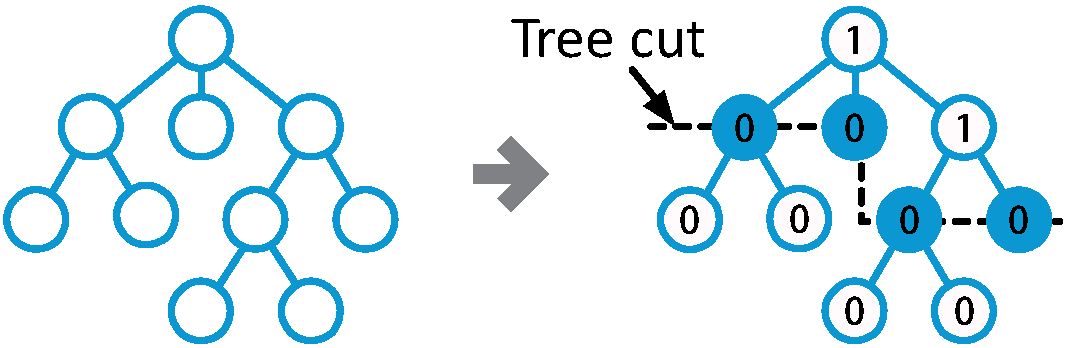
\includegraphics[width=2.5in]{fig/treecut}
  %\vspace{-mm}
  \caption{
%  \small
%  Tree cut example: the cut is denoted by the dotted line. Every node above the dotted line is labeled 1, while the rest are labeled 0.
Tree cut example: the cut is denoted by the dotted line. Every node above the dotted line is labeled 1, while the \docpr{others} are labeled 0.
}
  \label{fig:treecutexample}
  \vspace{-5mm}
\end{figure}



%The basic principle behind determining a set of optimal tree cuts is that each tree cut in the sequence should be similar to the one at the previous time point if the tree structures are similar (smoothness).
The basic principle \kg{to determine} a set of optimal tree cuts is that each tree cut in the sequence should be similar to the one at the previous time step if the tree structures are similar (smoothness).
%The tree cut must also adequately represent user interest and the topic tree at that time point (fitness).
The tree cut must also adequately represent user interests and the topic tree at that time step (fitness).
%Here the optimal tree cut is the cut that leads to the best similarity to the focus node(s) and the best representation for the tree (fitness).
%One straightforward method is to manually label all the tree cuts.
%Unfortunately, this method requires the user to examine every path from the root to a leaf to select a proper cut node.
%As a result, it \shixia{requires knowledge and skills and is very time-consuming,} especially when there are hundreds of topic trees and each of which contains hundreds of or even thousands of nodes.
%The global evolutionary tree cut algorithm developed in~\cite{cui2014} computes all the tree cuts together, based on the seed tree cut.
The global tree cut algorithm developed in~\cite{cui2014} computes all tree cuts \kg{simultaneously} based on the focused nodes.
%There are two problems when applying it to the text stream.
\kg{Two} problems arise when applying \kg{the aforementioned algorithm} to the text stream.
%First, it is very time consuming if we compute all the tree cut again when the new text data arrives.
First, it is very time consuming \docpr{to} compute all the tree \docpr{cuts each time} new text data arrives.
%First, \kg{computing} all the tree \kg{cuts once more} when new text data arrive \kg{is time-consuming}.
%Second, if the tree cuts are computed again with the new data, the existing tree cuts will be changed to some extent, which is difficult for analyst to maintain their visual momentum~\cite{Woods1984}.
%Second, if the tree cuts are computed again with new data, \kg{then} the existing tree cuts \kg{are} changed to \kg{a certain} extent, which \kg{makes maintaining the} visual momentum \kg{of analysts difficult}~\cite{Woods1984}.
%Second, if the tree cuts are computed again with \dc{the} new data, \kg{then} the existing tree cuts \kg{are} changed to \kg{a certain} extent, which \kg{makes maintaining the} visual momentum \dc{of analysts difficult}~\cite{Woods1984}.
Second, if the tree cuts are \docpr{recomputed along} with \dc{the} new data, \kg{then} the existing tree cuts \kg{are} changed to \kg{a certain} extent, which \kg{makes maintaining the} mental map \dc{of analysts difficult}~\cite{Woods1984}.


\begin{figure}[t]
  \centering
  % Requires \usepackage{graphicx}
  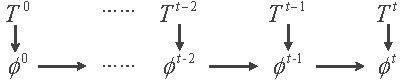
\includegraphics[width=2.1in]{fig/hmm2}
  \caption{
  %The dynamic Bayesian network for deriving streaming tree cuts.
  Dynamic Bayesian network for deriving streaming tree cuts. Here $T^t$ and ${\phi}^t$ are the topic tree and tree cut at \emph{t}.
  }\label{fig:hmm}
  \vspace {-5mm}
\end{figure}


\begin{table}[b]
\small
    \vspace{-5mm}

    \centering
    \scalebox{0.8}{

    \begin{tabular}{|c|c|}
    \hline
    %Data & Time span & N\_num & T\_num & Depth & I\_num \\
    \textbf{Notation} & \textbf{Definition} \\
   % Notation & Definition \\
    \hline
   %\multicolumn{2}{|c|}{Symbols} \\
   %\hline
   	$T^t$ & The topic tree at time $t$ \\
   \hline
	$\phi^t$ & The tree cut at time $t$ \\
	\hline
	$m$ & Number of focus nodes selected by the user \\
	\hline
	$T_{fi}$ &  The $i$th focus node \\
	\hline
	$\mathcal{D}_{fi}$ &  The document set of the $i$th focus node\\
	\hline	
	$ p({\phi}^t|{\phi}^{t-1},T^t)$ & The conditional distribution of $\phi^t$ according to DBN \\
	\hline
	$p({\phi}^t|T^t)$ & \tvcgminor{Fitness of tree cut ${\phi}^t$ to $T^t$} \\
	\hline
	$p({\phi}^t|{\phi}^{t-1})$ & Smoothness between adjacent tree cuts $\phi^t$ and $\phi^{t-1}$ \\
   \hline	
   	\tvcgminor{$p({\phi}^t|\mathcal{D}_{f0}, ..., \mathcal{D}_{fm})$} & The posterior probability of a tree cut ${\phi}^t$ \\
	\hline   	
	$E_1(T^t)$ & The similarity energy of the topic tree $T^t$ \\
   	\hline	
	$T_r$, $T_s$ &  A topic node (an internal node) in the topic tree \\
	\hline	   	
   	$\mathbf{S}(T_r,T_s)$ & The cosine similarity between topic nodes $T_r$ and $T_s$ \\
   	\hline	
	$l_s$ &  The label (0 or 1, see Fig.~\ref{fig:treecutexample}) of topic node $T_s$  \\
	\hline	
   	$E_2(\phi^{t}, \phi^{t-1})$ & The smoothness energy between tree cuts $\phi^t$ and $\phi^{t-1}$ \\
   	\hline	   	
	$\mathcal{D}_s$ &  The document set of topic node $T_s$\\
	\hline	
    $f_{DCM}(\mathcal{D})$  & The marginal distribution of document set $\mathcal{D}$ \\	
	\hline
	$\mathbf{WS}(T_c)$ &  Window size for $T_c$ in mean-shift clustering \\
	\hline
   %\multicolumn{2}{|c|}{Functions} \\
   %\hline
    \end{tabular}
    }
       \caption{
    \tvcgminor{Frequently used notations in the model.} %Sec.~\ref{sec:tree-cut}.}
    }
     \label{table:notations}
%   \vspace{-5mm}
\end{table}

%To solve these problems, we adopt a dynamic Bayesian network (DBN) to infer the tree cut for the incoming text data that is organized by a topic tree.
%To solve \kg{the aforementioned} problems, we adopt a dynamic Bayesian network (DBN) model to infer the tree cut for the incoming text data organized by a topic tree.
To solve \kg{the aforementioned} problems, we \docpr{have adopted} a dynamic Bayesian network (DBN) model to infer the tree cut for the incoming text data organized by a topic tree.
%Previous studies have shown that adopting overlapping successive views to support continuity across data sets is a frequently adopted principle for processing temporal data~\cite{Chakrabarti2006,Woods1984}.
Previous studies have shown that adopting overlapping successive views to support continuity across data sets is a frequently adopted principle \kg{to process} temporal data~\cite{Chakrabarti2006,Woods1984}.
%In our case, the new tree cut ${\phi}^t$ is relevant to the tree cuts adjacent to it in time as well as $T^t$ (Fig.~\ref{fig:hmm}).
In our case, the new tree cut ${\phi}^t$ is relevant to temporally \kg{adjacent} tree cuts as well as $T^t$ (Fig.~\ref{fig:hmm}).
%Specifically, topic mapping between adjacent trees is utilized as a constraint to smoothen the tree cut transitions over time.
\kg{In particular}, topic mapping between adjacent trees is utilized as a constraint to \dc{smooth} tree cut transitions over time.
%Based on this principle, we adopt  \looseness=-1
%The algorithm involves three steps: 1) users specify one or more topic nodes as the focus node(s); 2) the seed tree cut(s) is generated based on the user selected focus topic(s) and a posterior probability distribution; 3) a set of evolving tree cuts are derived based on the seed tree cut(s).

%For the sake of simplicity, we take one focus node as an example to illustrate the evolving tree cut algorithm.

\subsection{Model}

%In this section, we study the problem of identifying a set of coherent tree cuts in the topic trees given a small number of user-selected focus nodes.

%After deriving the seed tree cuts, we then propagate them to other topic trees, including the new coming topic trees, to generate a set of coherent tree cuts.
%The problem of tree cut propagation can be formulated as a labeling problem, in which the topic nodes above the tree cut are labeled 1 and the rest (including the cut nodes) are labeled 0 (Fig.~\ref{fig:treecutexample}).


\begin{figure*}[t]
\centering
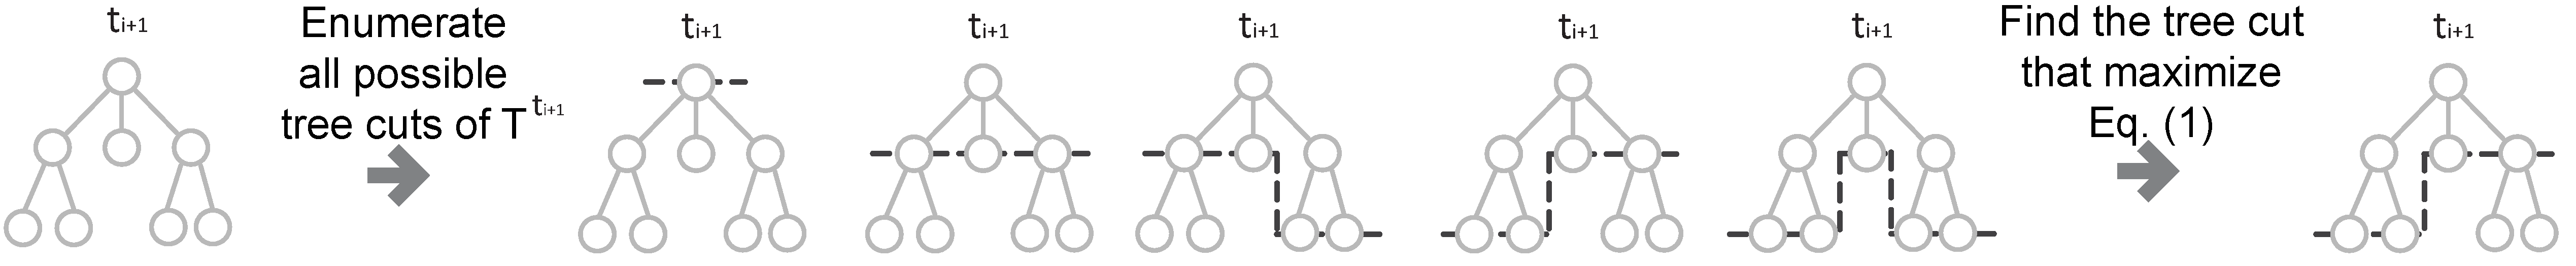
\includegraphics[width=0.9\textwidth]{fig/treecutalgorithm2}
\caption{\tvcgminor{Streaming tree cut algorithm: given the incoming topic tree $T^{t_{i+1}}$, we enumerate all possible tree cuts of $T^{t_{i+1}}$ and then pick the tree cut that maximizes Eq.~(\ref{eq:hmm1}).}}
\vspace{-5mm}
\label{fig:treecutalgorithm}
\end{figure*}


%Assume we already have a sequence of topic trees and the corresponding tree cuts based on users' interest, the problem of deriving the new tree cut in a text stream can be regarded as a labeling problem.
Assume \kg{that} we already have a sequence of topic trees and the corresponding tree cuts.
\kg{The} problem of deriving \kg{a} new tree cut in a text stream can \kg{then} be regarded as a labeling problem.
%In the labeling, the topic nodes above the tree cut are labeled 1 and the rest (including the cut nodes) are labeled 0 (Fig.~\ref{fig:treecutexample}).
\kg{The} topic nodes above the tree cut are labeled 1\kg{, whereas} the rest (including the cut nodes) are labeled 0 (Fig.~\ref{fig:treecutexample}).
We first introduce some frequently used notations in Table~\ref{table:notations}, which are useful for subsequent discussions.
%\tvcgminor{Table~\ref{table:notations} summarizes the notations commonly used in this section.}

%as an HMM.
%Given $m$ focus nodes \{${T_{fi}}$\} with document sets \{$\mathcal{D}_{fi}$\}, we aim to infer the tree cut ${\phi}^t$ in the new coming topic tree $T^t$.
%Given $m$ focus nodes \{${T_{fi}}$\} with document sets \{$\mathcal{D}_{fi}$\}, we infer the tree cut ${\phi}^t$ in the new coming topic tree $T^t$.
Given \emph{\normalsize m} focus nodes \{${T_{fi}}$\} with document sets \{$\mathcal{D}_{fi}$\}, we infer the tree cut ${\phi}^t$ in the \dc{incoming} topic tree $T^t$.
%In deriving the optimal tree cut, we consider both fitness (likelihood) and the expected node number that can be accommodated by the display area.
%As shown in Fig.~\ref{fig:hmm}, $T^t$ is an observation and ${\phi}^t$ is a hidden variable.
Fig.~\ref{fig:hmm} \kg{shows that} $T^t$ is an observation \kg{variable} and ${\phi}^t$ is a hidden variable.
%The relationship between ${\phi}^t$ and ${\phi}^{t-1}$ as well as $T^t$ can be modeled by DBN.
The relationship between ${\phi}^t$ and \docpr{${\phi}^{t-1}$, as well as $T^t$, can} be modeled by DBN.
Accordingly, the conditional distribution of ${\phi}^t$ is $p({\phi}^t|{\phi}^{t-1},T^t)$.
%On the other hand, ${\phi}^t$ is relevant to $\mathcal{D}_{f0},\mathcal{D}_{f1}, ..., \mathcal{D}_{fm}$ at each time $t$, we then formulate the inference of the new tree cut as
Since ${\phi}^t$ is relevant to $\mathcal{D}_{f0},\mathcal{D}_{f1}, ..., \mathcal{D}_{fm}$ at each time $t$, we formulate the inference of the new tree cut as:

\vspace{-5mm}
\begin{equation}
max\ p({\phi}^t,{\phi}^{t-1}, ...,{\phi}^0|\mathcal{D}_{f0},\mathcal{D}_{f1}, ..., \mathcal{D}_{fm})\cdot p({\phi}^t|{\phi}^{t-1},T^t).
\label{eq:hmm1}
\end{equation}


%\begin{figure*}
%\centering
%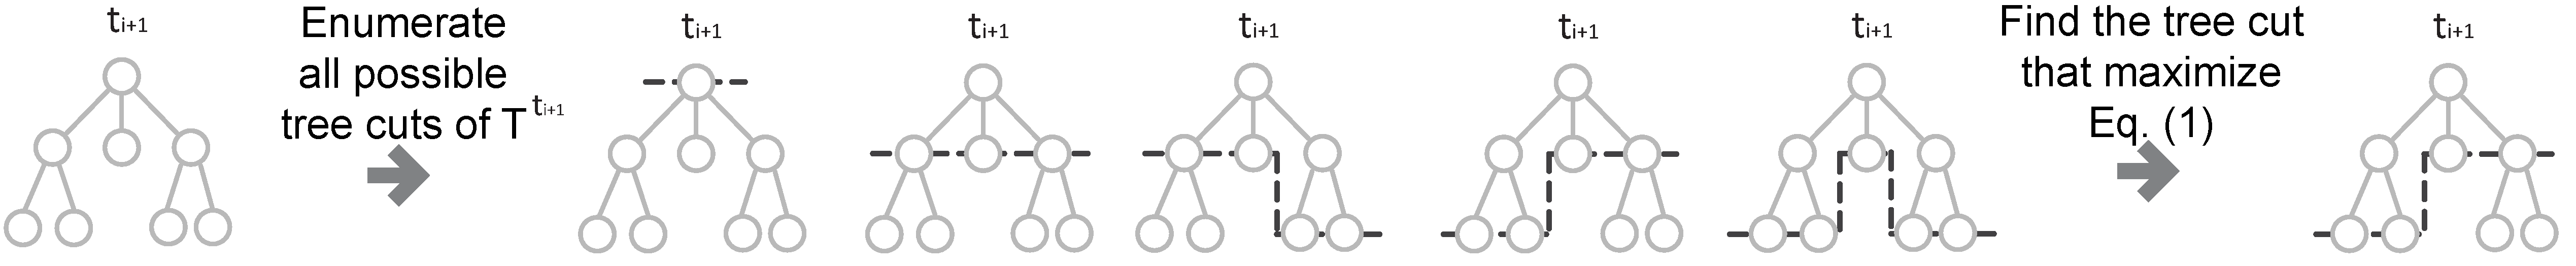
\includegraphics[width=0.9\textwidth]{fig/treecutalgorithm2}
%\caption{\tvcgminor{Streaming tree cut algorithm: given the incoming topic tree $T^{t_{i+1}}$, we enumerate all possible tree cuts of $T^{t_{i+1}}$ and then select the tree cut that maximizes Eq.~(\ref{eq:hmm1}).}}
%\vspace{-5mm}
%\end{figure*}

\tvcgminor{As shown in Fig.~\ref{fig:treecutalgorithm}, the goal is to find the tree cut that maximizes Eq.~(\ref{eq:hmm1}).
%Next, we describe how to calculate Eq.~(\ref{eq:hmm1}).
}

%Given $\mathcal{D}_{f0},\mathcal{D}_{f1}, ..., \mathcal{D}_{fm}$, ${\phi}^t, {\phi}^{t-1}, ..., {\phi}^0$ are conditionally independent, Eq.~\ref{eq:hmm1} can be rewritten as
%Given $\mathcal{D}_{f0},\mathcal{D}_{f1}, ..., \mathcal{D}_{fm}$, ${\phi}^t, {\phi}^{t-1}, ..., {\phi}^0$ are conditionally independent, Eq.~\ref{eq:hmm1} can be rewritten as
Since ${\phi}^t, {\phi}^{t-1}, ..., {\phi}^0$ are conditionally independent given $\mathcal{D}_{f0},\mathcal{D}_{f1}, ..., \mathcal{D}_{fm}$,
the first term is computed by $\prod\limits_{\tau=0}^{t}p({\phi}^\tau|\mathcal{D}_{f0},\mathcal{D}_{f1}, ..., \mathcal{D}_{fm})$.
According to the graphical model of DBN (Fig.~\ref{fig:hmm}), the second term is proportional to $p({\phi}^{t}|T^{t})p({\phi}^{t}|{\phi}^{t-1})$.
\xiting{Because} ${\phi}^{t-1},\ {\phi}^{t-2},...,\ {\phi}^{0}$ are known, Eq.~(\ref{eq:hmm1}) can be simplified as:
%\begin{equation}
%\small
%max\ \prod_{\tau=0}^{t}p({\phi}^{\tau}|\mathcal{D}_{f0},\mathcal{D}_{f1}, ..., \mathcal{D}_{fm})p({\phi}^{\tau}|T^{\tau})\prod_{\tau=1}^{t}p({\phi}^{\tau}|{\phi}^{\tau-1}).
%\label{eq:hmm1.5}
%\end{equation}
%%Here $p({\phi}^t|T^t)$ denotes how well the tree cut ${\phi}^t$ represents $T^t$, which is measured by the similarity energy $\mathbf{E}_1$:

\vspace{-4mm}
\begin{equation}
%\small
max\ p({\phi}^t|T^t)p({\phi}^{t}|{\phi}^{t-1})p({\phi}^{t}|\mathcal{D}_{f0},\mathcal{D}_{f1}, ..., \mathcal{D}_{fm}).
\label{eq:hmm2}
\end{equation}

$p({\phi}^t|T^t)$ denotes how well the tree cut ${\phi}^t$ represents $T^t$, which is measured by the similarity energy $\mathbf{E}_1$ in the form of $p({\phi}^t|T^t) = e^{-E_1(T^t)}$.
%$\mathbf{E}_1$ measures the content similarity of each topic $T_r$ in $T^t$ to the two topic sets, which are topic nodes sets labeled 0 and 1 respectively.
$\mathbf{E}_1$ measures the content similarity of each topic $T_r$ in $T^t$ \docpr{for} the two topic sets, which are topic \docpr{node} sets labeled 0 and \docpr{1, respectively}.
%It can be derived as follows:

\vspace{-3mm}
\begin{equation}
\small
E_1(T^t) = \sum_{T_r\in{\mathcal{N}^t}}\min_{T_s\in{\mathcal{N}^t},l_s=l_r}(-\log(\mathbf{S}(T_r,T_s))),
\end{equation}
where $l_r$ is the label (1 or 0) of topic node $T_r$, $\mathcal{N}^t$ is the set which contains all tree nodes in $T^t$.
%Similarity energy $\mathbf{E}_1$ measures the content similarity of topic $T_r$ to the two topic sets, \{1\} and \{0\}.
%\{1\} and \{0\} represent the nodes with fixed labels as 1 and 0.
%\{1\} and \{0\} represent \dc{nodes} with \dc{the} fixed labels \dc{1} and 0.
%At this step, they only contain the topic nodes in the key topic tree, as they are the only nodes with fixed labels.
%It measures the cost of node $r$ to the key label model built from the key tree cut.
%For a topic $T_r$, cosine similarity $\mathbf{S}(T_r,T_s)$ is used to compute the similarity value between $T_r$ and each topic $T_s$ in \{1\} or \{0\}.
For a topic $T_r$, \kg{the} cosine similarity $\mathbf{S}(T_r,T_s)$ is used to compute the similarity value between $T_r$ and $T_s$ with the same label.

$p({\phi}^t|{\phi}^{t-1})$ measures the smoothness cost between two adjacent tree cuts using the smoothness energy $\mathbf{E_2}$, which is defined as $p({\phi}^t|{\phi}^{t-1})= e^{-E_2(\phi^t,\phi^{t-1})}$. $\mathbf{E_2}$ measures the mapping similarity between $T^t$ and $T^{t-1}$:
\vspace{-3mm}
\begin{equation}
E_2(\phi^t,\phi^{t-1}) = \sum\limits_{T_r\in{\mathcal{N}^t},T_s\in{\mathcal{N}^{t-1}}}|l_r-l_s|\varphi(l_r,l_s),
\label{eq:hmm5}
\end{equation}
where $\varphi(l_r,l_s)$ denotes the mapping weight computed by the evolutionary tree clustering model.


%we calculate its similarity values to all the nodes in the key topic tree and treat the minimum one as its similarity value to the .
%Particularly, $\mathbf{E}_1(x_r)$ is defined as:
%\kg{In particular}, $\mathbf{E}_1(x_r)$ is defined as:
%
%\small
%\[
%\mathbf{E}_1(x_r)=
%    \begin{cases}
%    	0,     &\text{if  $T_r\in\{x_r\}$;}\\
%        \infty,&\text{if  $T_r\in\{1-x_r\}$;}\\
%        \min_{T_r\in\{x_r\}}(-\log(\mathbf{S}(T_r,T_s))), & \text{otherwise.}\\
%    \end{cases}
%\]
%\normalsize
%, $\mathcal{T}$ represents all the topics in the tree sequence,

%$p({\phi}^t|{\phi}^{t-1})$ measures the smoothness cost between two adjacent tree cuts.
%$p({\phi}^t|\mathcal{D}_{f0},\mathcal{D}_{f1}, ..., \mathcal{D}_{fm})$ is defined as a posterior probability of a tree cut ${\phi}^t$
$p({\phi}^t|\mathcal{D}_{f0},\mathcal{D}_{f1}, ..., \mathcal{D}_{fm})$ is defined as a posterior probability of a tree cut ${\phi}^t$\kg{. Thus,}
%and $p({\phi}^t)$ indicates the prior preference of the node number for the tree cut, which are defined as below.

%\subsubsection{Seed Tree Cut}
%we utilize a posterior probability to derive the optimal tree cut for a tree.
%Thus, we formulate the posterior probability of a tree cut $\phi$ as
\vspace{-5mm}
\begin{equation}
\label{eq:seed}
p({\phi}^t|\mathcal{D}_{f0}, \mathcal{D}_{f1}, ..., \mathcal{D}_{fm}) \propto p(\mathcal{D}_{f1}, \mathcal{D}_{f2}, ..., \mathcal{D}_{fm}|{\phi}^t) p({\phi}^t),
\end{equation}
where $p(\mathcal{D}_{f0}, \mathcal{D}_{f1}, ..., \mathcal{D}_{fm}|{\phi}^t)$ is the likelihood of the tree cut.
$p({\phi}^t)$ indicates the prior preference of the node number for the tree cut.
The tree cut that results in maximum posterior probability is the optimal tree cut.
%In our model, we derive the optimal tree cut(s) in the tree(s) that the focus node(s) belong to and regard them as the seed tree cut(s).
%We select such a tree cut because it can adequately represent the information needs of the user.

$p({\phi})$ is defined as $e^{-\lambda|\mathcal{C}_{{\phi}}|}$, where $\mathcal{C}_{{\phi}}$ is the set of topics in ${\phi}$, $|\mathcal{C}_{\phi}|$ is the node number in the tree cut, and $\lambda$ is the parameter that balances the
likelihood and expected node number.\looseness=-1

%We then illustrate how to calculate the likelihood of a tree cut.  for shixia
We then illustrate how the likelihood of a tree cut \kg{can be calculated}.
%We adopt a prediction model to estimate the likelihood of every possible tree cut.
We adopt a prediction model to estimate the likelihood of \kg{each} possible tree cut.
%For simplicity, we begin with one focus node. %with document set $\mathcal{D}_f$.
For simplicity\dc{'s sake}, we begin with one focus node. %with document set $\mathcal{D}_f$.
%\kg{We} begin with one focus node \kg{for simplicity}. %with document set $\mathcal{D}_f$.
%Given a focus node $T_f$ and its corresponding document set $\mathcal{D}_f$, the predictive probability of a tree cut $\phi$ is defined as
Given a focus node $T_f$ and its corresponding document set $\mathcal{D}_f$, the predictive probability of a tree cut $\phi$ is defined as: %\kg{follows:}
\begin{equation}
%\small
p(\mathcal{D}_f|\phi) = \sum_{T_s\in \mathcal{C}_{\phi}} \omega_s p(\mathcal{D}_f|\mathcal{D}_s),
\end{equation}
where $\mathcal{C}_{\phi}$ is the set of topics in $\phi$ and $\omega_s$ is the prior probability that all the documents in $\mathcal{D}_f$ belong to $\mathcal{D}_s$.
To calculate $\omega_s$, we assume that the probability of a set of documents belonging to a specific topic is proportional to the number of documents in that topic~\cite{Blundell2011}.
%\kg{We assume} that the probability of a set of documents \kg{belonging to} a specific topic is proportional to the number of documents in that topic \kg{to calculate $\omega_S$}~\cite{Blundell2011}.
Accordingly, we obtain $\omega_s = {|\mathcal{D}_s|}/{|\mathcal{D}_a|}$.
%$\mathcal{D}_a$ includes all documents in the tree.
$\mathcal{D}_a$ includes all documents in \kg{a} tree.
%$p(\mathcal{D}_f|\mathcal{D}_S)$ is the predictive distribution of the corresponding topic model
$p(\mathcal{D}_f|\mathcal{D}_s)$ is the predictive distribution of the corresponding \xiting{topic model.}
\begin{equation}
\small
p(\mathcal{D}_f|\mathcal{D}_s) = {f(\mathcal{D}_f \cup \mathcal{D}_s)}/{f(\mathcal{D}_s)},
\end{equation}
where $f(\mathcal{D})$ is the marginal probability of data $\mathcal{D}$.

%Dirichlet compound multinomial (DCM) distribution is derived based on multinomial and Dirichlet conjugate distributions~\cite{Liu2012, RasmusMadsen2005}.
\kg{The} Dirichlet compound multinomial (DCM) distribution is derived \kg{from} multinomial and Dirichlet conjugate distributions~\cite{Liu2012a}.
%Considering that DCM relies on hierarchical Bayesian modeling techniques, it is a more appropriate generative model than the traditional multinomial distribution for text documents.
%Considering that \kg{it} relies on hierarchical Bayesian modeling techniques, \kg{DCM} is a more appropriate generative model than the traditional multinomial distribution for text documents.
\dc{Because} \kg{it} relies on hierarchical Bayesian modeling techniques, \kg{DCM} is a more appropriate generative model than the traditional multinomial distribution for text documents.
%Thus, we utilize the DCM distribution to represent the marginal distribution $f(\mathcal{D})$ .
Thus, we utilize the DCM distribution to represent the marginal distribution $f(\mathcal{D})$ \kg{as follows:}
\begin{equation}
\label{eq:dcm}
%\small
f_{DCM}(\mathcal{D}) =  \prod_i^n \frac{(\sum_j^{|\mathcal{V}|}z_i^{(j)})!}{\prod_j^{|\mathcal{V}|} z_i^{(j)}!} \cdot \frac{\Delta({\bm \alpha}+\sum_i\bold{z}_i)}{\Delta({\bm \alpha})},
\end{equation}
where \xiting{$|\mathcal{V}|$ is the vocabulary size, $\bold{z}_i\in \mathcal{R}^{|\mathcal{V}|}$ is the word vector of the $i$th document, and $z_i^{(j)}$ is the frequency of the $j$th term.} % in the $i$th document
%${\bm \alpha} = (\alpha^{(1)},\alpha^{(2)},\ldots,\alpha^{(|\mathcal{V}|)})^T \in \mathcal{R}^{|\mathcal{V}|}$ is the parameter that controls the Dirichlet distribution, which is the prior of the multinomial distribution of each topic.
${\bm \alpha} = (\alpha^{(1)},\alpha^{(2)},\ldots,\alpha^{(|\mathcal{V}|)})^T \in \mathcal{R}^{|\mathcal{V}|}$ is the parameter that controls the Dirichlet distribution, which is the prior of the multinomial distribution of each topic.
$\Delta({\bm \alpha})$ is the Dirichlet delta function defined by $\Delta({\bm \alpha}) =\Gamma(\sum_{j=1}^{|\mathcal{V}|} \alpha^{(j)})/\prod_{j=1}^{|\mathcal{V}|} \Gamma(\alpha^{(j)})$.
%Here the Gamma function has the property $\Gamma(x+1) = x\Gamma(x)$.
\kg{The gamma} function has the property $\Gamma(\alpha+1) = \alpha\Gamma(\alpha)$.

We then extend the likelihood formulation to any number of focus nodes.
%When several focus nodes are selected, the predictive probability of a tree cut is
When several focus nodes are selected, the predictive probability of a tree cut is \kg{as follows:}
\begin{equation}
\small
p(\mathcal{D}_{f1}, \mathcal{D}_{f2}, ..., \mathcal{D}_{fm}|\phi) = \prod_{i\in [1, m]} p(\mathcal{D}_{fi}|\phi).
\end{equation}
%Directly maximizing the above predictive probability is intractable; thus, we adopt the tree pruning procedure of~\cite{He2003} for optimal tree cut selection.
Directly maximizing the \kg{aforementioned} predictive probability is intractable; thus, we adopt the tree pruning procedure \kg{presented in}~\cite{He2003} for optimal tree cut selection.



%\subsubsection{Streaming Tree Cut}

\subsection{Postprocessing}
%With the evolving tree cut algorithm, a set of representative topic nodes is selected to represent the topic tree at each time point.
\kg{A} set of representative topic nodes is selected to represent the topic tree at each time step.
\kg{using the evolving tree cut algorithm}.
However, two issues remain.
%First, the resulting tree cuts may still not ideally reflect the user's interests because a topic node could have any number of children.
First, the resulting tree cuts \kg{may not} ideally reflect \kg{user interests} because a topic node \kg{can} have any number of children.
%For example, a topic node that is highly related to the focus node may have many less related siblings.
For example, a topic node that is highly related to the focus node \kg{can} have many \kg{less-related} siblings.
%Considering that a tree cut cannot include the highly related node and its parent simultaneously, all its siblings have to be included in the tree cut as well.
Considering that a tree cut cannot \kg{simultaneously} include \kg{a} highly related node and its parent, all \kg{of} its siblings have to be included in the tree cut as well.
%This condition will result in showing less-related content with unnecessary details.
This condition \kg{results} in showing less-related content with unnecessary details.
%Second, in many cases, the number of representative topics at some time points is still too large to be displayed in the limited screen area.\looseness=-1
Second, the number of representative topics at \kg{several} time steps is still too large to be displayed in the limited screen area \kg{in many cases}.\looseness=-1


To address these issues, we propose a postprocessing approach to further reduce the topic number.
%\kg{We} propose a postprocessing approach to reduce the topic number \kg{further to address these issues}.
%It aims at (1) encouraging the merging of related siblings with similar content and less related to the focus nodes, (2) discouraging the merging of topics that highly related to the focus nodes, and (3) maintaining the smoothness between adjacent topic sets over time.\looseness=-1
%\kg{This approach} (1) \kg{encourages} the merging of related siblings with similar \kg{contents that are less} related to the focus nodes, (2) \kg{discourages} the merging of topics that \kg{are} highly related to the focus nodes, and (3) \kg{maintains} smoothness between adjacent topic sets over time.\looseness=-1
\kg{This approach} (1) \kg{encourages} the merging of related siblings with similar \dc{content that is less} related to the focus nodes, (2) \kg{discourages} the merging of topics that \kg{are} highly related to the focus nodes, and (3) \kg{maintains} smoothness between adjacent topic sets over time.\looseness=-1

To meet the aforementioned requirements, a clustering method is needed.
%\kg{A} clustering method is \kg{required to satisfy the aforementioned requirements}.
%Mean-shift clustering~\cite{comaniciu2002mean}, which automatically determines the cluster number, can easily be adapted to fulfill all the requirements.
Mean-shift clustering~\cite{comaniciu2002mean}, which automatically determines the cluster number, can \kg{be easily} adapted to fulfill all the requirements.
%The first requirement can be met by any clustering method. Thus, we focus on how to fulfill the others.\looseness=-1
The first requirement can be satisfied by any clustering method. Thus, we focus on how to fulfill the \kg{remaining requirements}.\looseness=-1

To meet the second requirement, an adaptive window size $\mathbf{WS}$ is defined for different clustering centers $T_c$.
%\kg{An} adaptive window size $\mathbf{WS}$ is defined for different clustering centers \kg{to satisfy the second requirement. That is,}
\begin{equation}
\small
	\mathbf{WS}(T_c)=
		\begin{cases}
			0 & \text{if } \mathbf{S}(\mathcal{D}_c, \mathcal{D}_f)\ge \gamma,\\
			{(\gamma-\mathbf{S}(\mathcal{D}_c, \mathcal{D}_f))w_{max}/\gamma} & \text{otherwise}.
		\end{cases}
\end{equation}
%$c$ is a non-focus node,
where $\gamma$ is the similarity threshold, $w_{max}$ is the maximum window size, and $\mathbf{S}(\mathcal{D}_c, \mathcal{D}_f)$ is the cosine similarity.
% between $\mathcal{D}_c$ and $\mathcal{D}_f$.\looseness=-1

To meet the third requirement, all the tree cuts are generated in temporal order.
%\kg{All} the tree cuts are generated in temporal order \kg{to satisfy the third requirement}.
Smoothness between adjacent topic sets is preserved by treating the previous clustering centers as the initial centers of the current cut node clustering.\looseness=-1
%\kg{The} smoothness between adjacent topic sets is preserved by using the previous clustering centers as the initial centers for clustering the current cut nodes.

%In this section, we demonstrate how to transform the data based on one single focus topic node.
%However, it can be easily extended to support multiple focus nodes.
%Briefly speaking, we run the whole algorithm for each focus node, and merge the results together.
%If there are conflicts between different results for the same topic tree, the finest cut nodes are chosen.
%Supporting multiple focus nodes is especially useful for comparing the topic evolution patterns between multiple topics users are interested in.

